\documentclass[a4paper,12pt,twoside]{memoir}

% Castellano
\usepackage[spanish,es-tabla]{babel}
\selectlanguage{spanish}
\usepackage[utf8]{inputenc}
\usepackage[T1]{fontenc}
\usepackage{lmodern} % Scalable font
\usepackage{microtype}
\usepackage{placeins}
\usepackage{listings}
\usepackage{subcaption}

\RequirePackage{booktabs}
\RequirePackage[table]{xcolor}
\RequirePackage{xtab}
\RequirePackage{multirow}
\usepackage{amssymb}

\widowpenalty10000
\clubpenalty10000
\newcommand{\myinput}[1]{%
	\begingroup%
	\renewcommand\normalsize{\tiny}% Specify your font modification
	\input{#1}%
	\endgroup%
}

% Códigos
\colorlet{punct}{red!60!black}
\definecolor{background}{HTML}{EEEEEE}
\definecolor{delim}{RGB}{20,105,176}
\colorlet{numb}{magenta!60!black}

\lstset{basicstyle=\normalfont\ttfamily,
	showstringspaces=false,
	commentstyle=\color{gray},
	keywordstyle=\color{numb},
	breaklines = true,
	resetmargins = true,
}

\lstdefinelanguage{bashb}{
	numbers=left,
	numberstyle=\scriptsize,
	stepnumber=1,
	numbersep=8pt,
	showstringspaces=false,
	breaklines = true,
	frame=lines,
	backgroundcolor=\color{background},
}

\lstdefinelanguage{json}{
	basicstyle=\normalfont\ttfamily,
	numbers=left,
	numberstyle=\scriptsize,
	stepnumber=1,
	numbersep=8pt,
	showstringspaces=false,
	breaklines = true,
	frame=lines,
	backgroundcolor=\color{background},
	literate=
	*{0}{{{\color{numb}0}}}{1}
	{1}{{{\color{numb}1}}}{1}
	{2}{{{\color{numb}2}}}{1}
	{3}{{{\color{numb}3}}}{1}
	{4}{{{\color{numb}4}}}{1}
	{5}{{{\color{numb}5}}}{1}
	{6}{{{\color{numb}6}}}{1}
	{7}{{{\color{numb}7}}}{1}
	{8}{{{\color{numb}8}}}{1}
	{9}{{{\color{numb}9}}}{1}
	{:}{{{\color{punct}{:}}}}{1}
	{,}{{{\color{punct}{,}}}}{1}
	{\{}{{{\color{delim}{\{}}}}{1}
	{\}}{{{\color{delim}{\}}}}}{1}
	{[}{{{\color{delim}{[}}}}{1}
	{]}{{{\color{delim}{]}}}}{1},
}

% Links
\usepackage[colorlinks]{hyperref}
\hypersetup{
	allcolors = {red}
}

% Ecuaciones
\usepackage{amsmath}

% Rutas de fichero / paquete
\newcommand{\ruta}[1]{{\sffamily #1}}

% Párrafos
\nonzeroparskip


% Imagenes
\usepackage{graphicx}
\newcommand{\imagen}[2]{
	\begin{figure}[!h]
		\centering
		\includegraphics[width=0.9\textwidth]{#1}
		\caption{#2}\label{fig:#1}
	\end{figure}
	\FloatBarrier
}

\newcommand{\imagenflotante}[2]{
	\begin{figure}%[!h]
		\centering
		\includegraphics[width=0.9\textwidth]{#1}
		\caption{#2}\label{fig:#1}
	\end{figure}
}



% El comando \figura nos permite insertar figuras comodamente, y utilizando
% siempre el mismo formato. Los parametros son:
% 1 -> Porcentaje del ancho de página que ocupará la figura (de 0 a 1)
% 2 --> Fichero de la imagen
% 3 --> Texto a pie de imagen
% 4 --> Etiqueta (label) para referencias
% 5 --> Opciones que queramos pasarle al \includegraphics
% 6 --> Opciones de posicionamiento a pasarle a \begin{figure}
\newcommand{\figuraConPosicion}[6]{%
  \setlength{\anchoFloat}{#1\textwidth}%
  \addtolength{\anchoFloat}{-4\fboxsep}%
  \setlength{\anchoFigura}{\anchoFloat}%
  \begin{figure}[#6]
    \begin{center}%
      \Ovalbox{%
        \begin{minipage}{\anchoFloat}%
          \begin{center}%
            \includegraphics[width=\anchoFigura,#5]{#2}%
            \caption{#3}%
            \label{#4}%
          \end{center}%
        \end{minipage}
      }%
    \end{center}%
  \end{figure}%
}

%
% Comando para incluir imágenes en formato apaisado (sin marco).
\newcommand{\figuraApaisadaSinMarco}[5]{%
  \begin{figure}%
    \begin{center}%
    \includegraphics[angle=90,height=#1\textheight,#5]{#2}%
    \caption{#3}%
    \label{#4}%
    \end{center}%
  \end{figure}%
}
% Para las tablas
\newcommand{\otoprule}{\midrule [\heavyrulewidth]}
%
% Nuevo comando para tablas pequeñas (menos de una página).
\newcommand{\tablaSmall}[5]{%
 \begin{table}
  \begin{center}
   \rowcolors {2}{gray!35}{}
   \begin{tabular}{#2}
    \toprule
    #4
    \otoprule
    #5
    \bottomrule
   \end{tabular}
   \caption{#1}
   \label{tabla:#3}
  \end{center}
 \end{table}
}

%
% Nuevo comando para tablas pequeñas (menos de una página).
\newcommand{\tablaSmallSinColores}[5]{%
 \begin{table}[H]
  \begin{center}
   \begin{tabular}{#2}
    \toprule
    #4
    \otoprule
    #5
    \bottomrule
   \end{tabular}
   \caption{#1}
   \label{tabla:#3}
  \end{center}
 \end{table}
}

\newcommand{\tablaApaisadaSmall}[5]{%
\begin{landscape}
  \begin{table}
   \begin{center}
    \rowcolors {2}{gray!35}{}
    \begin{tabular}{#2}
     \toprule
     #4
     \otoprule
     #5
     \bottomrule
    \end{tabular}
    \caption{#1}
    \label{tabla:#3}
   \end{center}
  \end{table}
\end{landscape}
}

%
% Nuevo comando para tablas grandes con cabecera y filas alternas coloreadas en gris.
\newcommand{\tabla}[6]{%
  \begin{center}
    \tablefirsthead{
      \toprule
      #5
      \otoprule
    }
    \tablehead{
      \multicolumn{#3}{l}{\small\sl continúa desde la página anterior}\\
      \toprule
      #5
      \otoprule
    }
    \tabletail{
      \hline
      \multicolumn{#3}{r}{\small\sl continúa en la página siguiente}\\
    }
    \tablelasttail{
      \hline
    }
    \bottomcaption{#1}
    \rowcolors {2}{gray!35}{}
    \begin{xtabular}{#2}
      #6
      \bottomrule
    \end{xtabular}
    \label{tabla:#4}
  \end{center}
}

%
% Nuevo comando para tablas grandes con cabecera.
\newcommand{\tablaSinColores}[6]{%
  \begin{center}
    \tablefirsthead{
      \toprule
      #5
      \otoprule
    }
    \tablehead{
      \multicolumn{#3}{l}{\small\sl continúa desde la página anterior}\\
      \toprule
      #5
      \otoprule
    }
    \tabletail{
      \hline
      \multicolumn{#3}{r}{\small\sl continúa en la página siguiente}\\
    }
    \tablelasttail{
      \hline
    }
    \bottomcaption{#1}
    \begin{xtabular}{#2}
      #6
      \bottomrule
    \end{xtabular}
    \label{tabla:#4}
  \end{center}
}

%
% Nuevo comando para tablas grandes sin cabecera.
\newcommand{\tablaSinCabecera}[5]{%
  \begin{center}
    \tablefirsthead{
      \toprule
    }
    \tablehead{
      \multicolumn{#3}{l}{\small\sl continúa desde la página anterior}\\
      \hline
    }
    \tabletail{
      \hline
      \multicolumn{#3}{r}{\small\sl continúa en la página siguiente}\\
    }
    \tablelasttail{
      \hline
    }
    \bottomcaption{#1}
  \begin{xtabular}{#2}
    #5
   \bottomrule
  \end{xtabular}
  \label{tabla:#4}
  \end{center}
}



\definecolor{cgoLight}{HTML}{EEEEEE}
\definecolor{cgoExtralight}{HTML}{FFFFFF}

%
% Nuevo comando para tablas grandes sin cabecera.
\newcommand{\tablaSinCabeceraConBandas}[5]{%
  \begin{center}
    \tablefirsthead{
      \toprule
    }
    \tablehead{
      \multicolumn{#3}{l}{\small\sl continúa desde la página anterior}\\
      \hline
    }
    \tabletail{
      \hline
      \multicolumn{#3}{r}{\small\sl continúa en la página siguiente}\\
    }
    \tablelasttail{
      \hline
    }
    \bottomcaption{#1}
    \rowcolors[]{1}{cgoExtralight}{cgoLight}

  \begin{xtabular}{#2}
    #5
   \bottomrule
  \end{xtabular}
  \label{tabla:#4}
  \end{center}
}

\graphicspath{ {./img/} }

% Capítulos
\chapterstyle{bianchi}
\newcommand{\capitulo}[2]{
	\setcounter{chapter}{#1}
	\setcounter{section}{0}
	\chapter*{#2}
	\addcontentsline{toc}{chapter}{#2}
	\markboth{#2}{#2}
}

% Apéndices
\renewcommand{\appendixname}{Apéndice}
\renewcommand*\cftappendixname{\appendixname}

\newcommand{\apendice}[1]{
	%\renewcommand{\thechapter}{A}
	\chapter{#1}
}

\renewcommand*\cftappendixname{\appendixname\ }

% Formato de portada
\makeatletter
\usepackage{xcolor}
\newcommand{\tutor}[1]{\def\@tutor{#1}}
\newcommand{\course}[1]{\def\@course{#1}}
\definecolor{cpardoBox}{HTML}{E6E6FF}
\def\maketitle{
  \null
  \thispagestyle{empty}
  % Cabecera ----------------
\noindent
\includegraphics[width=\textwidth]{cabecera}\vspace{1cm}%
  \vfill
  % Título proyecto y escudo informática ----------------
  \colorbox{cpardoBox}{%
    \begin{minipage}{.8\textwidth}
      \vspace{.5cm}\Large
      \begin{center}
      \textbf{TFG del Grado en Ingeniería Informática}\vspace{.6cm}\\
      \textbf{\LARGE\@title{}}
      \end{center}
      \vspace{.2cm}
    \end{minipage}

  }%
  \hfill\begin{minipage}{.20\textwidth}
    
\includegraphics[width=\textwidth]{escudoInfor}
  \end{minipage}
  \vfill
  % Datos de alumno, curso y tutores ------------------
  \begin{center}%
  {%
    \noindent\LARGE
    Presentado por \@author{}\\ 
    en Universidad de Burgos --- \@date{}\\
    Tutores: \@tutor{}\\
  }%
  \end{center}%
  \null
  \cleardoublepage
  }
\makeatother

\newcommand{\nombre}{José Luis Garrido Labrador} %%% cambio de comando
\newcommand{\titulo}{Aplicación de técnicas de minería de datos para la detección de crisis epilépticas y aplicación web}

% Datos de portada
\title{{\Huge SmartBeds}\\[0.5cm]\titulo}
\author{\nombre}
\tutor{Álvar Arnaiz González y José Francisco Díez Pastor}
\date{\today}

\begin{document}

\maketitle


\newpage\null\thispagestyle{empty}\newpage


%%%%%%%%%%%%%%%%%%%%%%%%%%%%%%%%%%%%%%%%%%%%%%%%%%%%%%%%%%%%%%%%%%%%%%%%%%%%%%%%%%%%%%%%
\thispagestyle{empty}


\noindent
\includegraphics[width=\textwidth]{cabecera}\vspace{1cm}

\noindent Dr. D. Álvar Arnáiz González, profesor del departamento de Ingeniería Civil, área de Lenguajes y Sistemas Informáticos.

\noindent Expone:

\noindent Que el alumno D. \nombre, con DNI 71707244Y, ha realizado el Trabajo final de Grado en Ingeniería Informática titulado <<SmartBeds - \titulo>>. 

\noindent Y que dicho trabajo ha sido realizado por el alumno bajo la dirección del que suscribe, en virtud de lo cual se autoriza su presentación y defensa.

\begin{center} %\large
En Burgos, {\large \today}
\end{center}

\vfill\vfill\vfill

% Author and supervisor
\begin{minipage}{0.45\textwidth}
\begin{flushleft} %\large
Vº. Bº. del Tutor:\\[2cm]
Dr. D. Álvar Arnaiz González
\end{flushleft}
\end{minipage}
\hfill
\begin{minipage}{0.45\textwidth}
\begin{flushleft} %\large
Vº. Bº. del co-tutor:\\[2cm]
Dr. D. José Francisco Díez Pastor
\end{flushleft}
\end{minipage}
\hfill

\vfill

% para casos con solo un tutor comentar lo anterior
% y descomentar lo siguiente
%Vº. Bº. del Tutor:\\[2cm]
%D. nombre tutor


\newpage\null\thispagestyle{empty}\newpage




\frontmatter

% Abstract en castellano
\renewcommand*\abstractname{Resumen}
\begin{abstract}
La epilepsia es una enfermedad que provoca crisis repentinas con convulsiones violentas y pérdidas del conocimiento. Ante estas situaciones es necesario suministrar unos primeros auxilios, sin embargo, durante las sesiones nocturnas es difícil detectar y tratar a tiempo estas crisis que pueden provocar daños graves a los pacientes que sufren esta enfermedad.

En este trabajo se investiga, a partir de datos reales provenientes de sensores en un colchón, métodos que puedan detectar situaciones de crisis en tiempo real de este modo, se podrá suministrar las atenciones necesarias con la mayor celeridad posible. 

Además de esto se ha creado una API REST y una página web que permite la gestión de camas (adición, borrado, edición), así como mostrar el estado actual de los sensores y las probabilidades de que el paciente esté sufriendo una crisis.
\end{abstract}

\renewcommand*\abstractname{Descriptores}
\begin{abstract}
Crisis epilépticas, minería de datos, desequilibrados, monitorización, clasificador, API REST.
\end{abstract}

\clearpage

% Abstract en inglés
\renewcommand*\abstractname{Abstract}
\begin{abstract}
Epilepsy is a disease whose symptoms are violent seizures and fainting. In these situations is necessary to apply first aid, but, overnight is difficult to detect and treat in time these crisis. That can cause serious damage to the patients. 

In this paper is researched, based on real data from sensors in a mattress, methods which can detect seizures in real time in such a way that caregivers can supply first aids as soon as possible.

In addition, it has been created a REST API and a website that allows the management of beds (creation, modification and elimination) as well as showing the current status of the sensors and the probabilities that the patient is suffering a crisis.
\end{abstract}

\renewcommand*\abstractname{Keywords}
\begin{abstract}
Epileptic seizures, data mining, unbalanced, monitoring, clasificator, API REST.
\end{abstract}

\clearpage

% Indices
\tableofcontents

\clearpage

\listoffigures

\clearpage

\listoftables
\clearpage

\mainmatter
\capitulo{1}{Introducción}

Gracias al avance de las técnicas y algoritmos de minería de datos, disciplinas no directamente relacionadas con la computación se han ido beneficiando de las ciencias de datos, a modo particular, la medicina está desarrollándose hacia modelos más preventivos gracias a las predicciones que se pueden generar utilizando estos métodos.

Es por este motivo que podemos ver en la literatura científica de los últimos años como se relaciona medicina y ciencia de datos, por ejemplo en estudios de detección de caídas~\cite{tolkiehn2011fall} o la motorización del sueño para la prevención de apneas~\cite{kortelainen2012sleepmonitoring}. En este trabajo de fin de grado, el objetivo es la detección de crisis epilépticas adscrito al proyecto homónimo vencedor del concurso universitario \textit{Desafío Universidad Empresa}~\cite{radio:radio_amiga_burgos_2018}

Aunque el análisis y detección de crisis epilépticas de manera automática ha sido ampliamente explorada por la comunidad científica esta se ha centrado o en el uso de pulseras inteligentes~\cite{ramgopal2014product_review} o el uso de encefalogramas~(\textit{EEG})~\cite{jeppesen2017modified,kumar2014epilepticeeg,tzallas2012review} para la predicción de estos eventos. Por tanto, ante pacientes con diversos problemas de salud que impiden el uso de pulseras y de dispositivos de control de actividad cerebral se realiza este proyecto que enfoca la detección de las crisis epilépticas en el uso de sensores de presión y biométricos en la cama donde duerme el paciente.

\section{Material adjunto}
Junto a esta memoria se incluyen:

\begin{itemize}
	\item \textbf{Cuaderno de investigación} con la evolución y pasos realizados durante la investigación junto con los resultados de cada experimento.
	\item \textbf{Anexos} donde se incluyen:
		\begin{itemize}
			\item Plan de proyectos
			\item Requisitos del sistema
			\item Diseño del sistema
			\item Manual para el programador
			\item Manual para el usuario
		\end{itemize}
	\item \textbf{API REST} en \textbf{Python-Flask}
	\item \textbf{Experimentos} en \textit{Jupyter Notebook}
\end{itemize}

Además se puede acceder a través de internet a la \href{https://ubu.joselucross.com}{ página web en producción} y al \href{https://github.com/jlgarridol/TFG-Smartbeds}{repositorio GitHub del proyecto}.
\capitulo{2}{Objetivos del proyecto}

Este apartado explica de forma precisa y concisa cuales son los objetivos que se persiguen con la realización del proyecto. Se puede distinguir entre los objetivos marcados por los requisitos del software a construir y los objetivos de carácter técnico que plantea a la hora de llevar a la práctica el proyecto.

\capitulo{3}{Conceptos teóricos}



\capitulo{4}{Técnicas y herramientas}

En este capítulo se encuentran las técnicas y herramientas utilizadas en el proceso de \textbf{investigación}, la creación del \textbf{servicio web} además de una sección con las \textbf{herramientas generales} usadas en todo el proyecto.

\section{Investigación}

El proyecto ha sido desarrollado aplicando diversas técnicas de minería de datos siguiendo el proceso KDD~\cite{ubu:mineria1} (Fig.~\ref{fig:kdd}). Aunque en esta memoria se explicará superficialmente, el desarrollo completo de la investigación se encuentra en el cuaderno de investigación adjuntado.

\begin{figure}
	\centering
	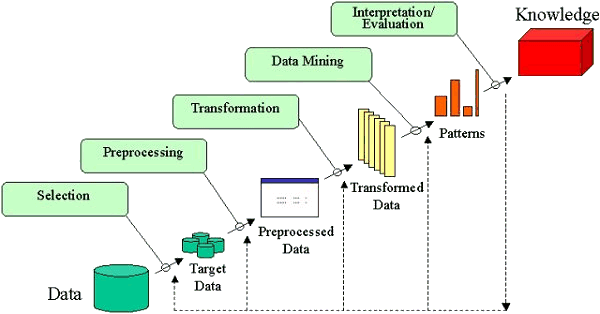
\includegraphics[width=\linewidth]{kdd}
	\caption{Flujo KDD~\cite{fayyad1996data}.}
	\label{fig:kdd}
\end{figure}

Para el proceso del clasificador final el flujo KDD ha sido el siguiente:

\begin{enumerate}
	\item \textbf{Selección}
		Los datos han sido cedidos por la asociación abulense \textit{PRONISA} que contiene jornadas nocturnas con identificadores de la cama, datos de presiones y datos vitales. Estos datos no están balanceados ya que existe una mayor cantidad de datos del paciente durmiendo que bajo una crisis epiléptica.
	\item \textbf{Preprocesado}
		Los datos se han limpiado reduciendo ruidos mediante filtros de señal.
	\item \textbf{Transformación}
		Se han generado datos estadísticos para series temporales que optimizaban el valor del área bajo la curva PCR~\cite{saito2015precision} desde los datos preprocesados.
	\item \textbf{Minería de datos}
		Se ha aplicado un sistema de clasificación doble, en primer lugar se utiliza un árbol de clasificación muy simple que divide entre las situaciones de despierto (bajas presiones en la cama) y acostado, en esta situación se aplica un clasificador \textit{Random Forest}~\cite{breiman2001random} para determinar si hay crisis o no.
	\item \textbf{Interpretación}
		Se ha desplegado una aplicación web con datos en tiempo real para evaluar de manera constante la situación actual del paciente.
\end{enumerate}

Este proceso de investigación se realizó sobre \textit{Python} utilizando el ecosistema de bibliotecas \textit{SciPy}~\cite{tool:scipy}, la biblioteca homónima se usó para crear filtros sobre los datos.

\paragraph{\textit{scikit-learn}~\cite{tool:scikit-learn}}biblioteca con funciones de aprendizaje automático para la creación de nuestros modelos.
\paragraph{\textit{NumPy}~\cite{tool:numpy}}biblioteca de computación especialmente útil para el almacenamiento de los datos y sus operaciones.
\paragraph{\textit{Pandas}~\cite{tool:pandas}}biblioteca de análisis de datos que usamos para almacenar los datos cargados desde los ficheros \textit{csv}.
\paragraph{\textit{MatPlotLib}~\cite{tool:matplotlib}}herramienta de dibujado usada para representar los datos y sus proyecciones.

Además, en algunas partes de la investigación se utilizó \textit{Weka}~\cite{tool:weka} para estudiar métodos que no se encontraban en \textit{scikit-learn} como el \textit{Random Balance}~\cite{diez2015random} o \textit{Rotation Forest}~\cite{rodriguez2006rotation}.

\section{Servicio web}

\subsection{\textit{Backend}}

Las herramientas utilizadas para programar el servidor han sido las siguientes:
\paragraph{Flask~\cite{tool:flask}}\textit{Microframwork} de código abierto (BSD) que ofrece una capa de abstracción muy alta de un servicio web, se utiliza para la creación de la lógica de negocio mediante la gestión de las rutas.
\paragraph{Jinja~\cite{tool:jinja}}Gestor de plantillas de código abierto (BSD) para Python, se utiliza para la creación de la interfaz web mediante la creación de páginas dinámicas en HTML.
\paragraph{Flask-SocketIO~\cite{tool:flask-socketio}}Integración del servicio de \textit{sockets}, \textit{Socket.IO}~\cite{tool:socketio}, compatible con los \textit{WebSockets}, se utiliza para la difusión de los datos en pacientes.
\paragraph{Gevent y Eventlet~\cite{tool:eventlet, tool:gevent}}Bibliotecas para el uso de tiempo real, asíncrono de hilos para el uso de \textit{Socket.IO}, el uso de estas bibliotecas es facilitar el procesado y difusión en tiempo real de los datos de los pacientes. 

Para la programación del sistema de hilos que distribuyen datos en tiempo real se siguieron los paradigmas de la programación orientada a objetos y de programación funcional. El sistema de rutas siguió las guías del \textit{microframework Flask}. 

Algunos patrones de diseño utilizados han sido el \textit{Singleton} para la API así como un \textit{Proxy} entre la interfaz web y la lógica de el API.

\subsection{\textit{Frontend}}

Para el desarrollo de la parte visible de la aplicación se han usado otra serie de herramientas:
\paragraph{Bootstrap~\cite{wiki:boostrap}}\textit{Framework} de \textit{CSS} de código abierto (MIT) creado por \textit{Twitter} para la creación de aplicaciones web redimensionables. Todos los estilos de la web se apoyan en este \textit{framework}.
\paragraph{jQuery~\cite{wiki:jquery}}\textit{Framework} de \textit{JavaScript} de código abierto (MIT) que simplifica el acceso al \textit{HTML DOM} de la página. La gestión de los eventos de la web se gestionan mediante este \textit{framework}.
\paragraph{Chart.js}Biblioteca de \textit{JavaScript} de código abierto (MIT) para la creación de grafos en \texttt{canvas}. Se usa para la visualización de las gráficas de presiones y constantes vitales.

\section{Herramientas generales}

Para el desarrollo general del proyecto se han utilizado las siguientes herramientas según el ámbito al que pertenecen:

\subsubsection{Servidor}
\paragraph{\textit{Nginx}}servidor web y de proxy reverso ligero de alto rendimiento~\cite{wiki:nginx} de código abierto (BSD simplificada).
\paragraph{\textit{MariaDB}}sistema de gestión de bases de datos derivado de \textit{MySQL}~\cite{wiki:mariadb} de código abierto (GPLv2). Este motor es extremadamente compatible con \textit{MySQL} porque es creado como una bifuración de esto para garantizar la existencia de este motor bajo GPL.
\paragraph{\textit{Proxmox}}es un entorno de virtualización de servidores~\cite{wiki:proxmox} de código abierto (AGPL). Su función principal es el despliegue y gestión de máquinas virtuales y contenedores.
\paragraph{\textit{Anarchy Arch}}sistema GNU/Linux derivado de \textit{ArchLinux}~\cite{wiki:arch} sobre el cual se ejecuta todo el servidor, está alojado en una máquina virtual del entorno \textit{Proxmox}.

\subsubsection{Miscelánea}
\begin{itemize}
	\item \textbf{Jupyter Notebooks}: IDE de programación de \textit{Python} basado en \textit{iPython} de código abierto (BSD).
	\item \textbf{PyCharm Professional}: IDE de programación para \textit{Python} avanzado basado en \textit{IntelliJ}.
	\item \textbf{Visual Studio Code}: Editor de código genérico de código abierto (MIT).
	\item \textbf{Postman}: IDE para la ejecución de request \textit{HTTP}.
	\item \textbf{Selenium}: IDE de pruebas sobre web de código abierto (APACHE).
	\item \textbf{CertBot}: Sistema para la firma \textit{SSL} sobre \textit{HTTP} gratuito de \textit{LetsEncrypt} de código abierto (MPL).
	\item \textbf{Overleaf}: Editor de \LaTeX{} online para el trabajo colaborativo.
	\item \textbf{\TeX{}Studio}: Editor de \LaTeX{} de código abierto (GPLv2).
	\item \textbf{Dia}: Editor de diagramas genérico de código abierto (GPL).
	\item \textbf{StartUML}: Editor de diagramas UML.
	\item \textbf{Codesketch DB}: Traductor bidireccional de código-diagrama para bases de datos.
	\item \textbf{Filezilla}: Aplicación para la trasferencia de ficheros sobre \textit{FTP} y \textit{SFTP} de código abierto (GPLv2).
	\item \textbf{GitHub}: Servicio online de \textit{hosting} para repositorios Git.
	\item \textbf{ZenHub}: Servicio online de integración de herramientas \textit{SCRUM} sobre GitHub.
\end{itemize}
\capitulo{5}{Aspectos relevantes del desarrollo del proyecto}
\section{Introducción}\label{cap:asp-rel}

En este capítulo se explicarán los aspectos más importantes tanto de la investigación, como del desarrollo. Los detalles más específicos y los resultados obtenidos se encuentran en los \textit{Anexos}. Además, se incluye un apéndice adicional con las fases y resultados de la investigación realizada, este se llama: \textit{Cuaderno de Investigación}.

\section{Investigación}

La fase de investigación ha ocupado la mayor cantidad de tiempo de este proyecto ya que ha sido también una introducción a la carrera investigadora. Ha sido desarrollada conjuntamente con Alicia Olivares Gil bajo la dirección de nuestros tutores el Dr. Álvar Arnáiz González y el Dr. José Francisco Díez Pastor.

El comienzo de esta investigación comenzó con un estudio del arte con el fin de conocer métodos y soluciones ya existentes y que hayan sido documentadas en la literatura científica. Sin embargo, la mayoría de artículos que existen actualmente para ese problema se centran en datos de encefalogramas, un tipo de datos que no poseemos. También exploramos problemas semejantes como detecciones de caídas mediante sensores de presión aunque la mayoría de estos sistemas se basaban en otros sensores como cámaras o acelerómetros. Algunos de estos artículos están resumidos en la sección~\ref{cap:trabrel}.

Tras esta exploración bibliográfica nos centramos en el estudio de los datos. Primero haciendo una limpieza eliminando datos con poca variabilidad, normalizarlos y eliminar datos ruidosos. Tras esto generamos proyecciones de los mismos a dos dimensiones tanto con datos limpiados, estadísticos o filtrados.

Los datos estadísticos que generamos en un comienzo fueron medias y desviaciones móviles de ventana $25$. Los filtros utilizados fueron el \textit{butterworth} y el \textit{savgol}, ambos de la librería \textit{SciPy}~\cite{tool:scipy}.

Las primeras conclusiones que obtuvimos era que los datos intermedios de las crisis documentadas tenían ciertas propiedades que las diferenciaba del resto, sin embargo esto se perdía a medida que se aumentaba la ventana del estudio. Además que este proceso era muy lento y necesitaba una gran cantidad de datos, por lo cual realmente podíamos obtener si hubo una crisis y no hacer una detección en directo.

A partir de aquí, para facilitar los procesos de preprocesado se crearon un conjunto de transformadores de datos que incluyen: un normalizador por característica como por grupos de las mismas, un filtro de ruido, un eliminador de características de poca varianza, un calculador de estadísticos móviles, un modificador del valor objetivo según una ventana temporal y dos compuestos que concatenan resultados o los convierte en una línea de tuberías de tal forma que se ejecuten secuencialmente.

Antes de pasar a la exploración de métodos para clasificar, acotamos las duraciones de las crisis que nos habían reportado, la primera razón es que la misma empresa nos informó de que los datos eran estimados y estos superaban el umbral para \textit{status epilepticus}~\cite{epilepsia}. Esta acotación se hizo analizando manualmente los datos dentro del rango que nos dieron determinando como crisis las situaciones con presiones anómalas. 

\subsection{Detección de anomalías}
Lo siguiente que se realizó fue un estudio de detección de anomalías en el cual se intentó tanto predecir una crisis a partir de entrenar un clasificador \texttt{OneClassSVM} entrenando con todos los datos de no crisis y también predecir una situación de no crisis entrenando el mismo clasificador con los datos de crisis.

Lo primero que obtuvimos es que una crisis es un subconjunto de una situación no crisis ya que el clasificador no lo detecta como anomalía al ser entrenado con las situaciones de no crisis.

El segundo obtenido fue que las diversas crisis no coexisten en el mismo espacio, ya que al entrenar el clasificador con una crisis determinaba como anomalía a todas las demás crisis al igual que al resto de datos. Además, en el caso de combinar dos situaciones de crisis el entrenamiento ya tiene un gran índice de fallo si los datos no son estadísticos (media y desviación).

Los resultados del entrenamiento se pueden ver en las tablas~\ref{tab:matriz-conf-1a} y~\ref{tab:matriz-conf-1a-2d} y los de test en las tablas~\ref{tab:matriz-test-2a} y~\ref{tab:matriz-test-3a}, en estás últimas se puede ver que la predicción siempre es errónea para un conjunto nuevo de datos.

\myinput{./research-book/train-tables.tex}
\myinput{./research-book/test-tables.tex}

\subsection{\textit{Ensembles} para desequilibrados}
Debido a que la detección de anomalías no dio resultados correctos, se pasó a hacer un estudio de clasificadores combinados (\textit{ensemble}) optimizados para la resolución de problemas con datos desequilibrados~\cite{diez2015diversity,galar2012review}.

Debido a que en el conjunto de datos ya habíamos hecho un submuestreo al limitar el conjunto de datos a los del día de las crisis probamos a hacer un sobremuestreo mediante SMOTE~\cite{galar2012review} con los algoritmos de \textit{Bagging}, \textit{AdaBoostM1} y \textit{Rotation Forest}~\cite{rodriguez2006rotation}.

Los resultados de este experimento fue que los clasificadores sobreajustaban los datos de las crisis y no eran capaces de predecir correctamente otras crisis. Además pudimos comprobar que el algoritmo de \textit{boosting} no predecía correctamente los datos de entrenamiento lo que, junto con el hecho de que la etiquetación sabíamos que había sido manual, da pie a la conclusión de que los datos están mal etiquetados~\cite{ubu:mineria3}.

También se probó a realizar una validación cruzada con todo el conjunto de datos usando el clasificador de \textit{Rotation Forest}~\cite{rodriguez2006rotation} obteniendo unos buenos resultados.

\subsection{Búsqueda de mejores características}
Otro proceso que se hizo fue la búsqueda de mejores características a partir de un análisis estadístico tratando a los datos como una serie temporal. A partir primero de la búsqueda de la mejor ventana temporal (obtenido el valor de noventa) mediante la optimización del valor del AUC~\cite{galar2012review} y de PRC~\cite{Davis2006RPR}. El desarrollo completo de esta búsqueda está explicado con mayor lujo de detalles en el Apéndice \textit{Cuaderno de Investigación} en el capítulo \textit{Extracción de características con tsfresh y clasificador Random Forest}.

\subsection{\textit{Ensembles} para desequilibrados - estadísticos de series temporales}
Para finalizar la investigación se volvieron a probar los \textit{ensembles} para conjuntos desequilibrados de Galar et. al.~\cite{galar2012review} y Díez et. al.~\cite{diez2015random, diez2015diversity} usando sobremuestreo con \textit{SMOTE}, submuestreo con \textit{RUS} y muestreo aleatorio con \textit{Random Balance}. Se usaron los clasificadores de comité aleatorio, \textit{bagging} y \textit{rotation forest}.

Los resultados fueron semejantes a la primera ocasión ya que el testeo con la otra crisis siempre obtenía un ratio de aciertos con las crisis de 0.

Los resultados se pueden ver en las tablas~\ref{tab:crisis1} y~\ref{tab:crisis2}

\begin{table}\scriptsize
	\begin{center}
		\begin{tabular}{llllllll}
			\toprule
			Algoritmo & TPR &          FPR &       TNR & FNR &       PRC &       AUC &       ACC \\
			\midrule
			RB - Bag                &   0 &            0 &         1 &   1 &  0.984425 &  0.552363 &   0.98178 \\
			RB - RC       &   0 &            0 &         1 &   1 &  0.981267 &  0.485675 &   0.98178 \\
			RB - RotF        &   0 &  1.65036e-06 &  0.999998 &   1 &  0.980551 &  0.485354 &  0.981778 \\
			RUS - Bag          &   0 &  0.000899444 &  0.999101 &   1 &  0.980613 &  0.447139 &  0.980897 \\
			RUS - RC &   0 &            0 &         1 &   1 &  0.981076 &    0.4806 &   0.98178 \\
			RUS - RotF  &   0 &  0.000394435 &  0.999606 &   1 &  0.982287 &  0.486412 &  0.981393 \\
			SM - Bag                         &   0 &  0.000173287 &  0.999827 &   1 &  0.984367 &  0.565807 &   0.98161 \\
			SM - RC                &   0 &            0 &         1 &   1 &  0.981278 &  0.486071 &   0.98178 \\
			SM - RotF                 &   0 &  1.56784e-05 &  0.999984 &   1 &  0.982673 &  0.512364 &  0.981764 \\
			\bottomrule
		\end{tabular}
		\caption{Métodos para desbalanceados - Entrenamiento con la primera crisis, testeo con la segunda crisis.}
		\label{tab:crisis1}
	\end{center}
\end{table}

\begin{table}\scriptsize
	\begin{center}
		\begin{tabular}{llllllll}
			\toprule
			Algoritmo & TPR &         FPR &       TNR & FNR &       PCR &       AUC &       ACC \\
			\midrule
			RB - Bag                &   0 &   0.0109634 &  0.989037 &   1 &  0.995225 &  0.491511 &  0.983616 \\
			RB - RC       &   0 &  0.00571683 &  0.994283 &   1 &  0.993912 &  0.446135 &  0.988834 \\
			RB - RotF        &   0 &  0.00488364 &  0.995116 &   1 &   0.99517 &  0.525534 &  0.989663 \\
			RUS - Bag          &   0 &   0.0461306 &  0.953869 &   1 &  0.994863 &  0.514533 &  0.948642 \\
			RUS - RC &   0 &   0.0112769 &  0.988723 &   1 &  0.994602 &  0.506568 &  0.983304 \\
			RUS - RotF  &   0 &   0.0128567 &  0.987143 &   1 &  0.994482 &  0.468075 &  0.981733 \\
			SM - Bag                         &   0 &    0.017596 &  0.982404 &   1 &  0.995505 &  0.539099 &   0.97702 \\
			SM - RC                &   0 &   0.0048424 &  0.995158 &   1 &  0.994052 &  0.458383 &  0.989704 \\
			SM - RotF                 &   0 &  0.00344412 &  0.996556 &   1 &  0.994742 &  0.502318 &  0.991094 \\
			\bottomrule
		\end{tabular}
		\caption{Métodos para desbalanceados - Entrenamiento con la segunda crisis, testeo con la primera crisis.}
		\label{tab:crisis2}
	\end{center}
\end{table}

\section{Desarrollo de la aplicación}
La fase de desarrollo ha ocupado alrededor de un cuarto del tiempo del proyecto. A su vez se ha dividido en cuatro partes: una primera de búsqueda de herramientas para la difusión en tiempo real de datos, una segunda de diseño, una tercera de implementación y finalmente el despliegue.

La primera parte fue la más corta, consistió en explorar herramientas que fueran compatibles con websocket~\cite{wiki:websocket} ya que este protocolo es el más eficaz para distribución en tiempo real de datos mediante HTTP, que es la tecnología más sencilla para la creación de una \textit{API}. La herramienta seleccionada fue \textit{socketIO}~\cite{tool:socketio} que daba una interfaz sencilla y multilenguaje.

\subsection{Diseño}
La fase de diseño fue la que más tiempo llevó de este apartado debido a que hubo que discutir muchos detalles con mi compañera Alicia Olivares Gil. El objetivo de esto era crear una interfaz sencilla y funcional para que pudiese desarrollar una aplicación Android lo más rápidamente posible.

El primer paso fue determinar los casos de uso, que debido a la limitación temporal, se resumieron lo más posible. Decidimos hacer una gestión de usuarios y camas con un sistema de permisos simplificado de forma tal que los usuarios pueden estar asociados a camas. También se creó un usuario maestro administrador que tuviese permisos sobre todo.

Otro punto importante fueron los datos. Los usuarios son formados por un identificador único, un nombre de usuario único, una contraseña y un token dinámico y único. Este último es el que permite identificar al usuario para realizar operaciones \textit{CRUD}. Este cambia por cada inicio de sesión del usuario de tal forma que solo puede existir una sesión abierta a la vez.

Las camas, por otro lado, están formadas por un par de identificadores de los sensores de presión (\textit{MAC}) y de los sensores biométricos (\textit{UUID}) que son usados también como el nombre del espacio donde se difundirán los datos de esa cama. También identifican a la cama un número secuencial y un nombre de la misma. Cada cama tiene a su vez una combinación de IP-puerto del rango de \textit{multicast} que especifica a la aplicación a donde tiene que escuchar. 

Como parte final del diseño se determinó cuales serían los pasos para el \textit{handshake} del proceso de obtención de datos en tiempo real. Se decidió que este sería una petición a la API para solicitar el espacio de nombres, luego una apertura de conexión a \textit{socketIO}, si la conexión era correcta lanzar una petición de solicitud de datos (\texttt{give\_me\_data}) para finalmente escuchar paquetes (\texttt{package}) al espacio de nombres solicitado.

\subsection{Implementación}
El último proceso fue la implementación, que se dividió en cuatro partes: primero la creación de la \textit{API REST} para la gestión de camas y de usuarios, la segunda fue la implementación de la difusión de datos en tiempo real, la tercera la creación de ventanas para la interacción vía web y por último la creación de test unitarios y de integración (interfaz).

\subsubsection{Implementación de la \textit{API}}
Esta \textit{API} se implementó utilizando dos partes, una primera como una clase \textit{singleton} que sirve de conexión a la base de datos y realiza las operaciones especificadas controlando los permisos y una segunda parte que hace de adaptador para traducir peticiones \textit{HTTP} a la signatura de las funciones de la clase.

El funcionamiento global de una petición es:
\begin{enumerate}
	\item Se hace una petición \texttt{POST} mediante \texttt{x-www-form-urlencoded} a la ruta de la operación deseada.
	
	\item La función asociada a la ruta desempaqueta el mensaje y crea una llamada al objeto de la \textit{API}.
	
	\item La \textit{API} realiza la operación solicitada y devuelve el resultado deseado.
	
	\item La función de adaptación recoge el resultado y crea un objeto de respuesta \textit{JSON} con un código \textit{HTTP} y un mensaje.
\end{enumerate}

En el caso de que alguno de los procesos fallasen, se generaría un código de error según el tipo de error. Si fuese 400 implicaría que la petición realizada no tiene los parámetros esperados, 401 si el valor del \textit{token} no está correctamente asociado, 403 si no se tuviesen permisos para realizar la operación, 404 si no existiese la operación deseada, 405 si se hace con un método erróneo, 418 si la operación no estuviese disponible por causa de la versión y 500 en el caso de que existiese un error en el servidor. Si todo fuese correcto el número del código sería 200. Todos estos valores provienen del estándar RFC~7231~\cite{RFC7231}.

\subsubsection{Difusión en tiempo real}
Para poder hacer la difusión en tiempo real se necesita de la librería de \texttt{flask-socketio}~\cite{tool:flask-socketio} y de \texttt{gevent}~\cite{tool:gevent}. 

El primer paso es crear los hilos del \textit{pipeline} del procesamiento de los datos (uno de escucha y otro de procesado). Esto se hace usando la interfaz \texttt{Thread} pero compatibilizado con \texttt{gevent} mediante un \textit{monkey patching}~(explicado en la sección~\ref{cap:mokey}).

El proceso completo de creación de hilos se puede ver en el Anexo \textit{Manual del programador}, la estructura de su colaboración se puede ver en el diagrama de clases de la figura~\ref{fig:classes}.

\begin{figure}
	\centering
	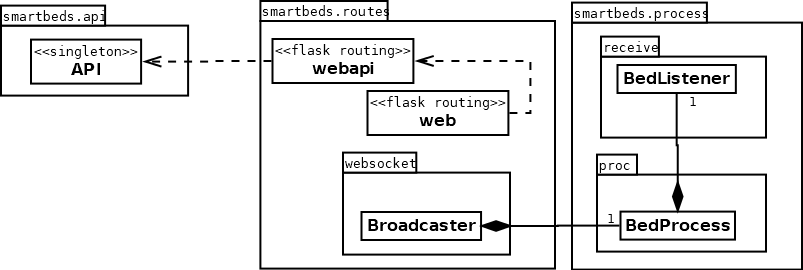
\includegraphics[width=\textwidth]{classes}
	\caption{Diagrama de clases.}
	\label{fig:classes}
\end{figure}

Tras esto es necesario crear las capturas de eventos de \textit{socketIO} para poder detectar cuando se solicitan datos y enviarlos. Este envío se hace mediante otro hilo, el de difusión que emite por \textit{broadcast} a todos los clientes de cada cama. Estos hilos funcionan solo dentro del entorno de petición (\textit{request context}) por lo que morían al cerrar el usuario la conexión, por tanto, para evitar que los datos se acumulasen en el servidor se usaron colas en los hilos de procesamiento con un tamaño máximo a la ventana temporal~(90) de tal forma que se borrasen los más viejos si entraban nuevos datos.

Un detalle importante es que, como los datos no podemos tenerlos en tiempo real, ya que pertenecen a la empresa que nos los suministra. Por ello hemos simulado un \textit{streaming} de datos local usando UDP emitiendo una nueva línea del CSV cada $0.4$ segundos, que es una estimación del intervalo por el cual nos llegan los datos.

Otra modificación sobre el diseño ha sido que realmente existe una única cama y las distintas camas que existen realmente usan los mismos hilos ya que los \textit{Broadcaster} realmente emiten a todos los \textit{namespaces} que existen. Se ha hecho esto debido a las limitaciones técnicas del equipo de despliegue ya que cada cama implicaba una serie de tres hilos que ralentizan mucho el sistema.

También se utiliza actualmente un clasificador aleatorio por intervalos de tal manera que cambie la probabilidad de crisis cada noventa instancias entre los tres estados posibles: crisis, no crisis, despierto; con el fin de poder probar como cambian las interfaces en los distintos estados, sobre todo porque el clasificador obtenido al final no era capaz de predecir situaciones de crisis.

El resultado final en la aplicación web se puede ver en la figura~\ref{fig:man_bed}.

\begin{figure}
	\centering
	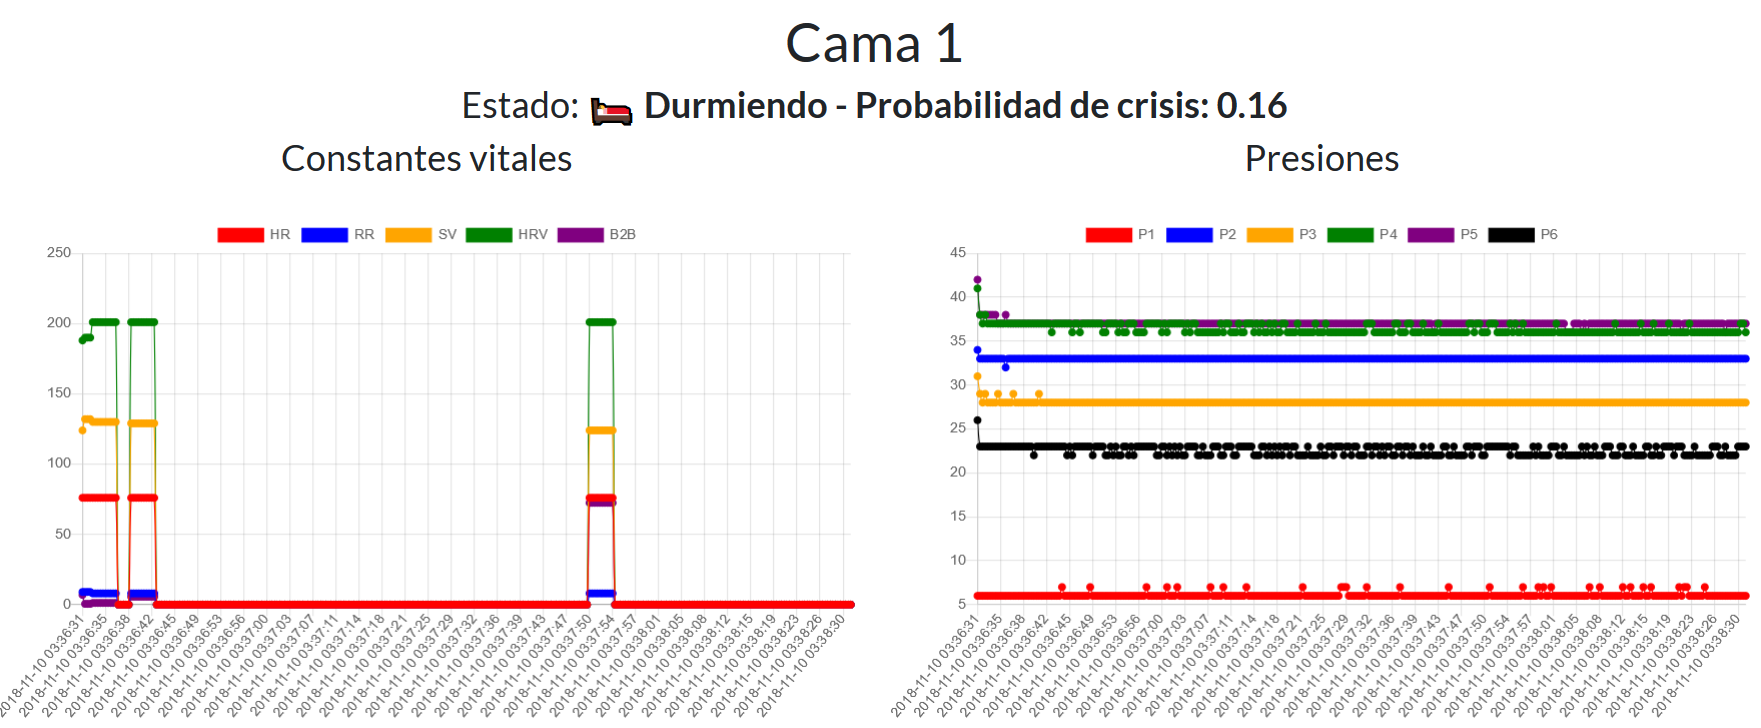
\includegraphics[width=\textwidth]{manual/man_cama1}
	\caption{Página con la información en tiempo real de una cama.}
	\label{fig:man_bed}
\end{figure}


\subsubsection{Ventanas \textit{HTML}}

La interfaz web de la aplicación se hizo mediante plantillas \textit{Jinja}~\cite{tool:jinja} de \textit{HTML}. Se apoyó con el \textit{framework} de \textit{boostrap 4}~\cite{wiki:boostrap} para el \textit{CSS} y \textit{jQuery} para la implementación de funciones \textit{JavaScript}.

Para facilitar este desarrollo se crearon varios componentes separados y una plantilla maestra de la que heredarán todas las páginas. Esto evita el código repetido así como facilita el desarrollo de la aplicación. Los componentes que se crearon fueron la barra de navegación, el pie de página, las funciones generales de para la validación de los formularios y un modal para mostrar los errores.

Otro aspecto importante del desarrollo de la interfaz fue la creación de los gráficos en tiempo real. Se usó la librería \textit{Graph.js} para hacer gráficos en objetos \texttt{canvas} de \textit{HTML}. En un primer momento la librería actualizaba muy lentamente, pero el problema estaba en la programación de los hilos de \textit{Python} con los hilos, esto se solucionó con la llamada \texttt{eventlet.sleep(0)} en el \texttt{Broadcaster} para que los datos fuesen en tiempo real.

Para optimizar el renderizado es estas gráficas se optó por eliminar las animaciones y los valores de \texttt{hover}\footnote{Evento al deslizar el puntero del ratón sobre el objeto.} para que no se ejecutasen nuevas llamadas a eventos del \texttt{DOM} que mostraban los datos de esa instancia temporal.

Otra tecnología que se usó en el desarrollo de la interfaz web fue el uso de llamadas asíncronas al servidor mediante \textit{AJAX}. De esta manera se pueden evitar cargas completas de la página de manera innecesaria. Especialmente en las situaciones que la operación no requería mostrar nuevos datos en la pantalla como la creación, modificación o borrado de usuarios y camas. 

\subsubsection{Pruebas}
Las pruebas consistieron en pruebas unitarias y de integración. Para las primeras se usó \texttt{unnittest} de \textit{Python} y para las de integración se hicieron test sobre la interfaz web con \textit{Selenium IDE}. Este por motivos de tiempo no se ha trasladado a código y se puede ejecutar importando el fichero .side al \textit{IDE} y ejecutarlo desde el mismo. En el Anexo \textit{Manual del Programador} este punto está más explicado.

Los test unitarios se basaron en un test parametrizado y un fichero \textit{JSON} con la configuración de todos los test deseados.
\\\\ %Para no dejar viudas
\begin{lstlisting}[language=JSON]
{
   "tests": [
      {
         "name": "nombre del test",
         "description": "descripcion del test",
         "func": "funcion de la clase API",
         "input": ["parametros de entrada en orden"],
         "output": ["salida esperada"],
         "excepts": "excepciones esperadas, si es null no se espera ninguna"
      },
      ...
   ],
   "tokens": 
      {
         "usuario": "token",
         ...
      }
}
\end{lstlisting}

Cada test tiene seis campos, un nombre y descripción para identificar al test, una función de la clase \texttt{smartbeds.api.API}, una entrada en el orden de los parámetros, la salida esperada (si espera una) y la excepción que espera (si espera una). También tiene una serie de tokens asociados a los usuarios, aunque ese campo es solamente útil para el programador de los test para saber que token está asociado a cada usuario.

Antes de ejecutar los tests se instala una base de datos de pruebas que borra la base de datos anterior.

\subsection{Despliegue}
El despliegue de la aplicación fue una de las partes más complicadas del proceso de desarrollo. En primer lugar se intentó desplegar sobre un dispositivo embebido, en particular la \textit{Raspberry Pi 2B}. Sin embargo, este \textit{hardware} no fue capaz de soportar el rendimiento necesario para enviar los datos en un tiempo real.

Por eso se traspasó el sistema a otro servidor personal\footnote{Este servidor forma parte del grupo \textit{JKA Network}} con varias máquinas virtuales llamado \textit{Al-Juarismi}. Se incorporó la base de datos a una de ellas de nombre \textit{V-Lovelace} y la lógica de la aplicación se almacenó en la máquina \textit{V-Babbage}. En esta última también se añadió la simulación de la cama como un demonio semejante al que se puede ver en el anexo del \textit{Manual del programador}.

Este servidor está configurado de tal forma que se requiera un certificado \textit{SSL} sobre todas las páginas que albergue. Por tanto se usó un certificado de \textit{LetsEncrypt} para el mismo.

\section{Test de usabilidad}

Para comprobar si la aplicación web realizada era usable e intuitiva se realizó un test de usabilidad\footnote{Se puede acceder en el enlace \url{https://forms.gle/oo9m3nmGA46UqMKv9}} junto a la aplicación móvil realizada por Alicia Olivares Gil. Para comprobarlo se propusieron cinco tareas a los usuarios:

\begin{enumerate}\small
	\item Iniciar sesión con el usuario y contraseña que le proporcionamos. 
	\item Cambiar la contraseña. 
	\item Consultar el estado de los pacientes. 
	\item Consultar las gráficas explicativas sobre el estado de los pacientes. 
	\item Cerrar sesión	
\end{enumerate}

Y para recoger las valoraciones se pidió la cumplimentación de un formulario con cuatro afirmaciones a valorar entre 1 y 5 siendo 1 \textit{completamente en desacuerdo} y 5 \textit{completamente de acuerdo}. Las afirmaciones eran:
\begin{itemize}\small
	\item \textit{Me ha resultado fácil realizar las tareas propuestas}.
	\item \textit{Me ha resultado fácil interpretar los elementos gráficos (iconos, botones, gráficas...)}.
	\item \textit{La selección de elementos gráficos usados en la aplicación (colores, tipografías...) me ha parecido acertada}.
	\item \textit{La aplicación me ha parecido muy buena}.
\end{itemize}

A estas afirmaciones, para facilitar la interpretación de los resultados, se les ha asignado una valoración equivalente cuyos nombres han sido: \textit{Facilidad de uso}, \textit{Interpretabilidad}, \textit{Uso de gráficos} y \textit{Global} respectivamente.

También se hizo una distinción entre el perfil profesional del encuestado entre \textit{tecnológico}, \textit{educación} y \textit{asistencia sanitaria}. El objetivo de esta distinción es poder comprobar si la aplicación es fácil de usar por el tipo de usuario al que va destinado (educadores y asistentes sanitarios). Se ha tomado como referencia las valoraciones de los usuarios de perfil técnico. 

\subsection{Resultados del test}
Se han recogido un total de doce votos, cinco de perfil tecnológico y tres de educación y cuatro de asistencia sanitaria (Fig.~\ref{fig:usab_prop}).

\begin{figure}
	\centering
	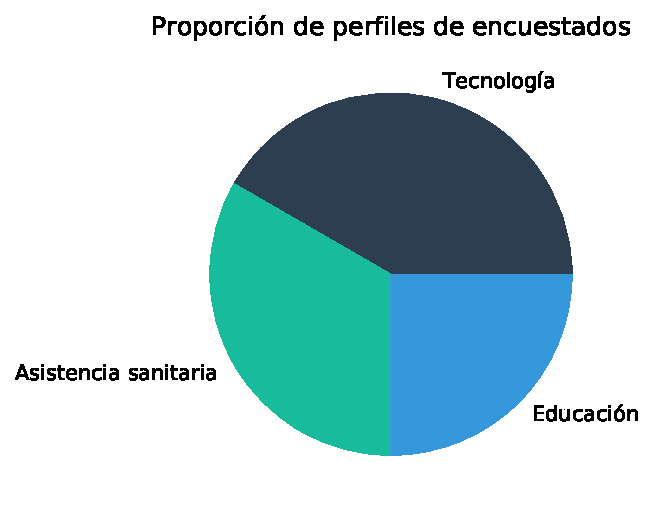
\includegraphics[width=0.6\textwidth]{usability/web_proportion.pdf}
	\caption{Proporción de encuestados según su perfil laboral}
	\label{fig:usab_prop}
\end{figure}

Podemos ver en la figura~\ref{fig:usab_global} las valoraciones generales de todos los encuestados. Se observa que la valoración general es muy positiva siendo la interpretabilidad de los datos el aspecto que peor valoración tiene. Sin embargo, la media es de $(3.5)$ que sigue por encima de la neutralidad de la valoración (un valor de $3$), podemos concluir que la aplicación es usable e intuitiva independientemente del perfil laboral del encuestado.

\begin{figure}
	\centering
	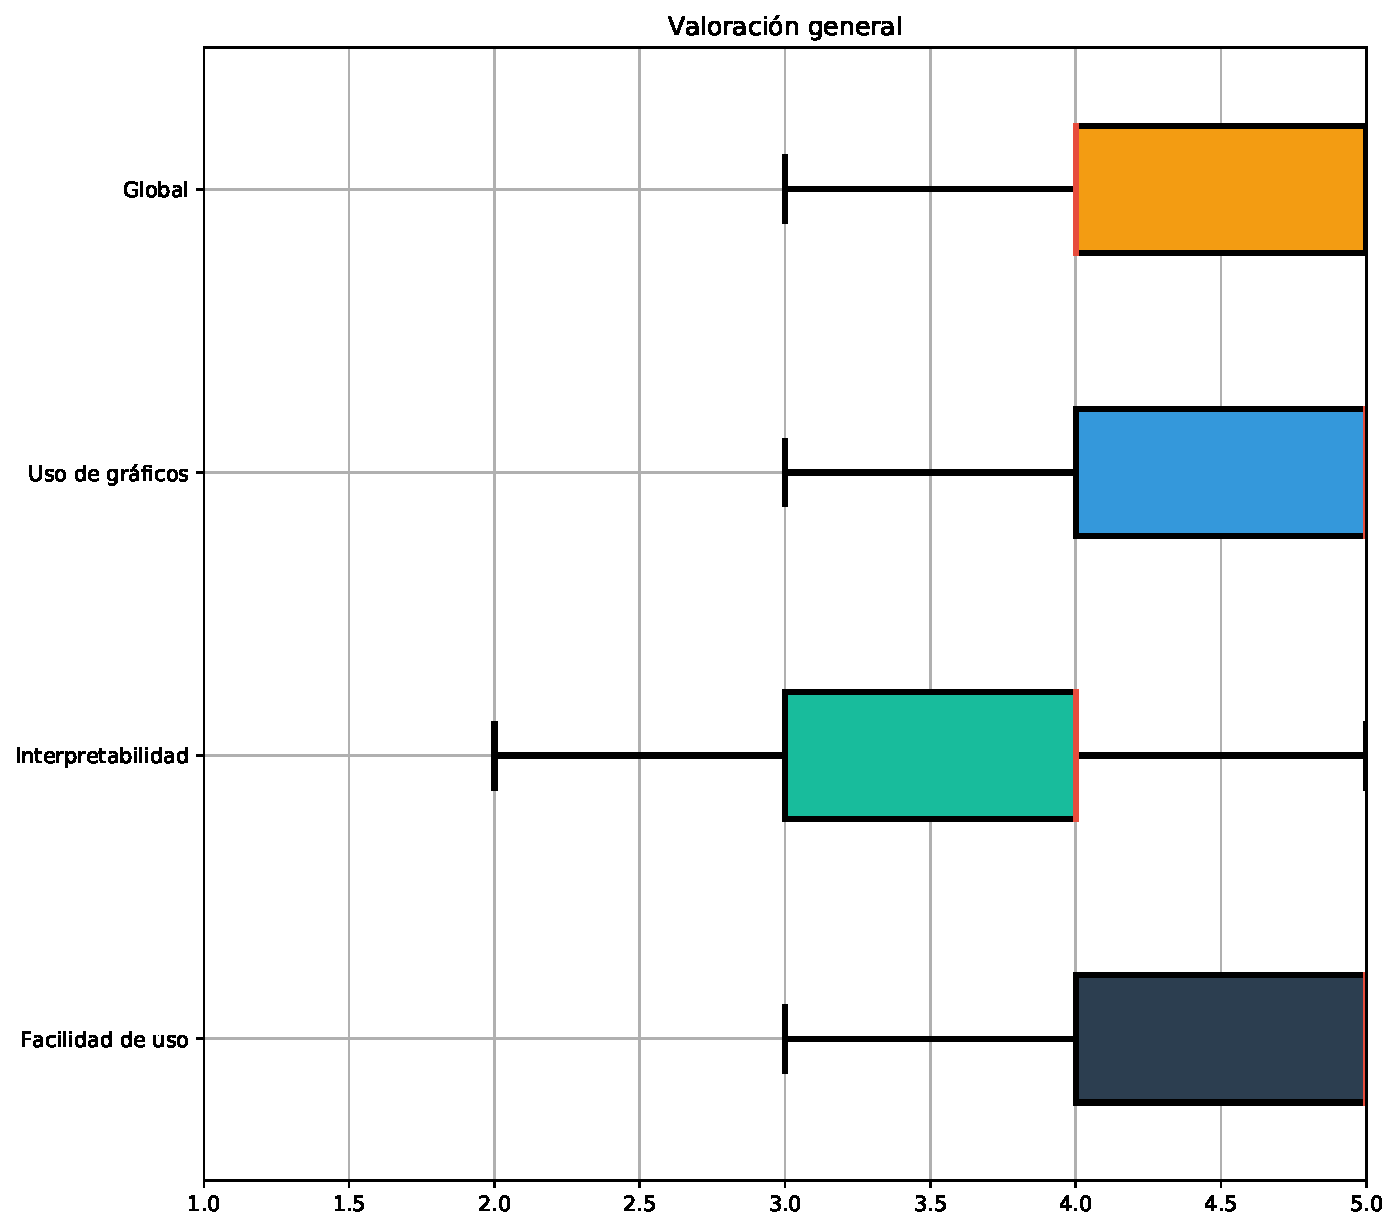
\includegraphics[width=\textwidth]{usability/web_general.pdf}
	\caption[Valoraciones de todos los encuestados.]{Valoraciones de todos los encuestados. El extremo izquierdo representa el valor más bajo y el extremo derecho el valor más alto. La caja representa la distribución de los valores del primer cuartil (izquierda), la mediana (linea roja) y tercer cuartil (derecha). La media es la mitad de la caja.}
	\label{fig:usab_global}
\end{figure}

Respecto a la comparativa entre el perfil \textbf{tecnológico} y el \textbf{no tecnológico} (Fig.~\ref{fig:usab_comp}) podemos observar que, aunque tanto la valoración global como la interpretabilidad por los usuarios \textbf{no tecnológicos} están más dispersas, siguen teniendo valores medios muy altos. Además, sus valoraciones tanto sobre el uso de gráficos como de la facilidad de uso es menos dispersa que la del grupo \textbf{tecnológico}.

Por todo esto podemos concluir que la aplicación es usable e intuitiva para el perfil al que está destinado y no ha habido ninguna tendencia en el desarrollo de hacer una aplicación excesivamente técnica lo que hubiese perjudicado la usabilidad de la misma.

\begin{figure}[h]
	\centering
	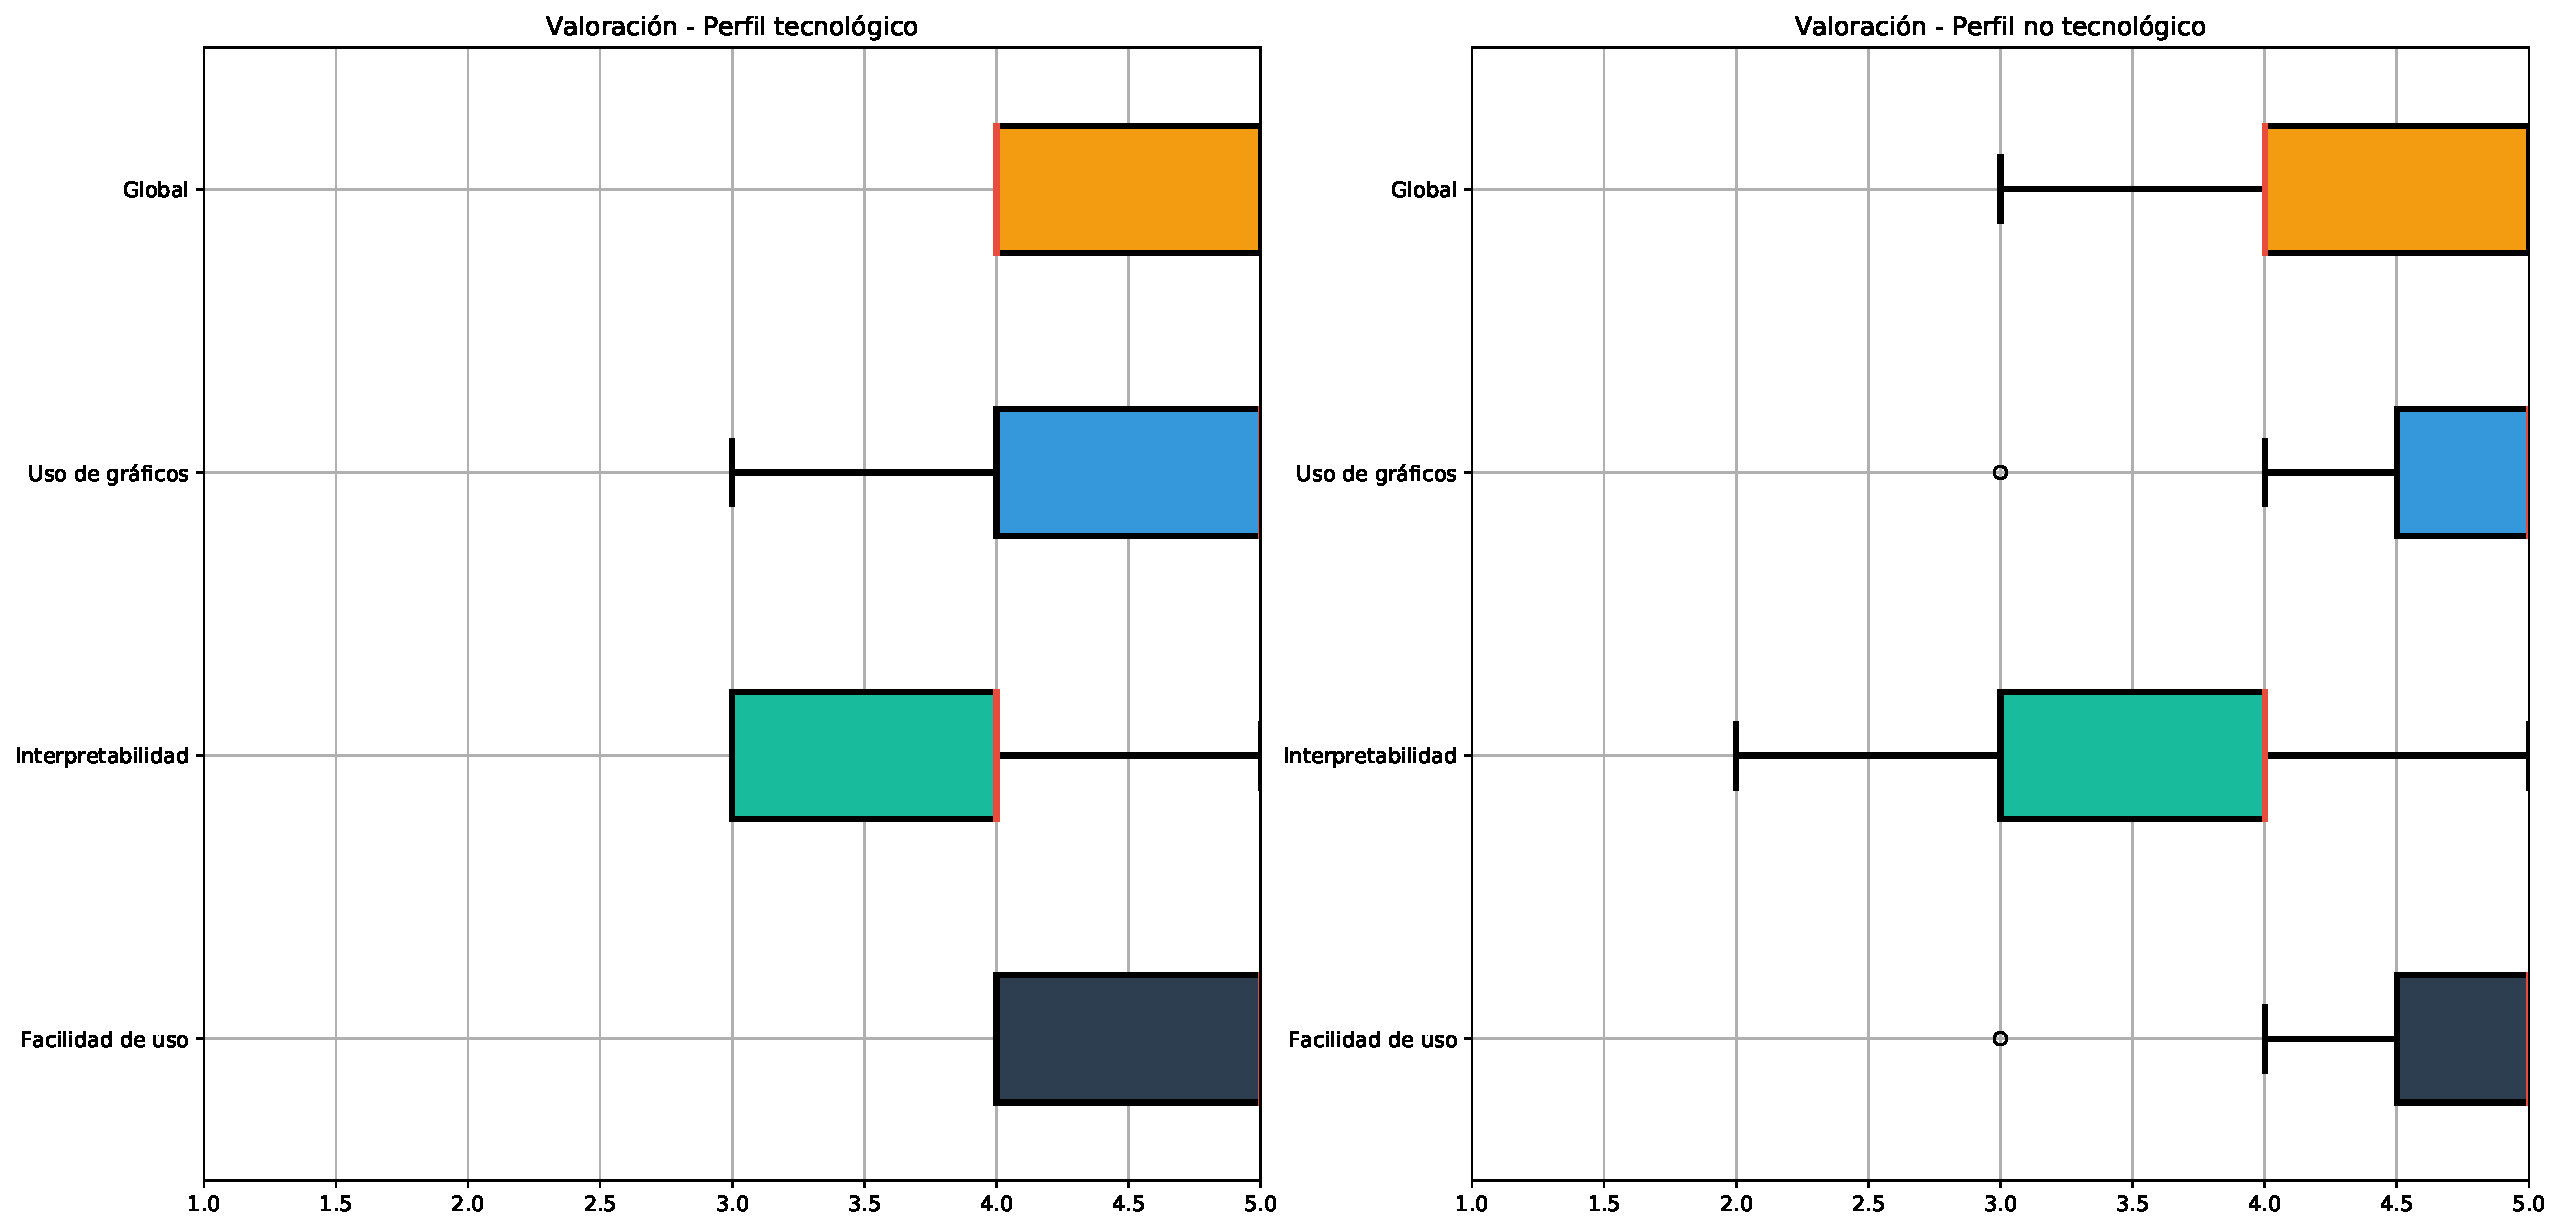
\includegraphics[width=\textwidth]{usability/web_comparation.pdf}
	\caption[Comparación de valoraciones entre perfil tecnológico y no tecnológico.]{Comparación de valoraciones entre perfil tecnológico y no tecnológico. El extremo izquierdo representa el valor más bajo y el extremo derecho el valor más alto. La caja representa la distribución de los valores del primer cuartil (izquierda), la mediana (linea roja) y tercer cuartil (derecha). La media es la mitad de la caja.}
	\label{fig:usab_comp}
\end{figure}

\section{\textit{Monkey Patching}}\label{cap:mokey}

También conocido como el parches de mono en español, es la técnica por la cual se extiende o modifica la funcionalidad del sistema de manera local y en ejecución. Solo se permite en lenguajes dinámicos como \textit{Python} o \textit{Ruby}~\cite{wiki:monkey_patch}.

Bajo esta definición las librerías \textit{Gevent}~\cite{tool:gevent} y \textit{Eventlet}~\cite{tool:eventlet} aportar una función de parcheo para cambiar las funciones de las librerías nativas de \textit{Python}: \texttt{sockets}, \texttt{dns}, \texttt{time}, \texttt{select}, \texttt{thread}, \texttt{os}, \texttt{ssl}, \texttt{httplib}, \texttt{subprocess}, \texttt{sys}, \texttt{aggresive}, \texttt{Event}, \texttt{builtins}, \texttt{signal} y \texttt{queue}.

Gracias a esto todas esas funciones y clases que no son compatibles con el sistema de eventos de \textit{socketIO} se pueden utilizar sin necesidad de aprender todas las funciones y clases alternativas de \textit{gevent} o \textit{eventlet}.

\section{Uso de \textit{CodeClimate}}
Para hacer un estudio de la calidad del código y hacer las modificaciones necesarias para que el código sea más mantenible, se ha utilizado \textit{CodeClimate} una herramienta que analiza gratuitamente proyectos de \textit{GitHub} de código abierto.

En el primer análisis se obtuvo una calificación de \textbf{\textit{F}}, siendo la peor nota posible. Sin embargo, esto fue debido a que se analizó partes del proyecto que no es propio como son las librerías de \textit{JavaScript} y los estilos \textit{CSS} que se han utilizado. Por ello se creó un fichero \texttt{.codeclimate.yml} para ignorar todo el código ajeno y se volvió a realizar un análisis.

El segundo análisis tuvo de calificación \textit{\textbf{C}}, que aunque no es la peor calificación, si que requiere una mejora del código para hacerlo más mantenible. Para ello se eliminó código repetido, que en su mayoría trataba de comprobaciones de la validez de las llamadas a las funciones (comprobación de tipos y de la sesión web). Para solucionar esto se incluyeron funciones que agrupasen las comprobaciones idénticas eliminando así el código repetido.

Una situación especial fue la creación de un \textit{decorador} para las funciones de las rutas de la web para que se ejecutase en todas las que se requiriese la inclusión del \texttt{token} del usuario en la sesión actual para poder redirigir correctamente estas peticiones. 

La última ejecución se obtuvo una calificación de \textit{\textbf{B}}. A partir de este punto es difícil de mejorar debido a que algunos errores detectados no son refactorizables. Estos son la gran cantidad de parámetros de algunas funciones, que no pueden ser modificadas al ser heredadas de otras librerías; la cantidad de métodos de la clase \texttt{API} que, al englobar toda la lógica de negocio, no tiene sentido partir en diferentes clases. 

\capitulo{6}{Trabajos relacionados}

En la introducción se han presentado diversos trabajos que sobre la detección de crisis epilépticas, a continuación se presentarán con más detalles el estado del arte en este campo.

\section{Artículos científicos}\label{cap:trabrel}
\subsection{\textbf{\textit{Epileptic seizure detection}}~\cite{schuyler2007epileptic}}
Este artículo de 2007 se centra en la detección de epilepsia y sus momentos previos mediante el uso de los datos de encefalograma (EEG) descompuesto con la transformada ondícula con redes \textit{RBF}. Exploran diversos conjuntos de características combinadas con diversas cantidades de neuronas obteniendo resultados de un $89\%$ de precisión media tanto en la detección de situaciones de crisis como de los momentos previos a una crisis.

Los datos usados han sido provenientes de ratas, en concreto dos sanas y cinco epilépticas de las cuales obtuvieron $2356$ segmentos de crisis.

\subsection{\textbf{\textit{Automated Epileptic Seizure Detection Methods: A Review Study}}~\cite{tzallas2012review}}
Este estudio de revisión del 2012 hace una compartativa de 45 artículos de métodos de detección de crisis epilépticas, siendo un punto muy importante para comenzar una exploración ya que incluye una gran bibliografía revisada. Contiene el proceso de extracción de características, todos probados con un conjunto de datos de encefalogramas, también documenta las precisiones obtenidas. 

\subsection{\textbf{\textit{Direction  Sensitive  Fall  Detection  Using  a  Triaxial  Accelerometer  and  aBarometric  Pressure  Sensor}}~\cite{tolkiehn2011fall}}
Otro artículo explorado es este de 2011 centrado en la detección de caídas debido a que se centra en entradas mediante presiones y acelerómetros. El objetivo de la investigación está tanto en la detección de la caía como en la dirección de la misma. 

El principal reto en este trabajo estaba en discriminar correctamente las situaciones que eran una caida de las que no debido a que no es lo mismo tumbarse en la cama, que caerse de la misma. 

El proceso que sigue es extraer características de los datos del acelerómetro obteniendo la amplitud y el ángulo del mismo, hacer dos procesos sobre estos como un árbol de decisión de tal manera que de concluir posible caída se para a un sensor de presión que determina si es una caída o no lo es.

La precisión de los resultados ronda el $85\%$ al incluir los sensores de presión mejorando en $4$ puntos al solo utilizar el acelerómetro.

\subsection{\textit{\textbf{Seizure detection, seizure prediction, and closed-loop warning systemsin epilepsy}}~\cite{ramgopal2014product_review}}

Este artículo se centra en una revisión de productos comerciales para la detección de crisis epilépticas así como diversos métodos para esta detección.

Presenta un rango de dieciséis años de estudios  con múltiples modelos y datos. La mayoría centrado en datos de encefalogramas y máquinas de vectores soporte. Entre el rango de productos que presenta la variedad del mercado sin tener en cuenta de que exista o no un artículos científicos sobre los mismos. Aunque la mayoría trata de \textit{wereables} como pulseras si que presenta algunos sistemas basados en camas.
\capitulo{7}{Conclusiones y Líneas de trabajo futuras}

Para finalizar la exposición de esta memoria se comentará en este capítulo las conclusiones del trabajo así como lineas futuras que se pueden realizar.

\section{Conclusiones}
De este proyecto se pueden obtener las siguientes conclusiones.
\begin{itemize}
	\item No se ha podido crear un modelo útil para la monitorización de pacientes con epilepsia por diversos motivos. El primero es la escasez de datos para el estudio ya que de todas las crisis documentadas solo teníamos datos de tres. Segundo, la etiquetación deficiente de las mismas ya que solo se poseía un rango temporal. En tercer lugar no se poseían datos de las constantes vitales o estos eran de mala calidad lo que impedía contrastar la información con datos médicos fiables.
	\item Los algoritmos de clasificación desarrollados en la universidad de Burgos, el \textit{Rotation Forest} y el \textit{Random Balance} han sido los que mejores resultados han dado para este problema, teniendo en cuenta que no ha existido ninguno probado que haya sido de predecir bien una crisis nueva.
	\item Los conjuntos de datos muy desbalanceados y muy ruidosos son difíciles de analizar. Más aún es encontrar modelos capaces de interpretarlos correctamente. Esto nos ha derivado en clasificadores que sobreajustan demasiado o que no son capaces de ajustar.
	\item Desarrollar la API usando el \textit{framework} \textit{Flask} para \textit{Python} ha facilitado el desarrollo gracias a su simplicidad, en especial gracias a que no se requieren unos grandes conocimientos de programación de servicios \textit{HTTP}.
	\item \textit{SocketIO} es una herramienta que ha resultado muy útil para hacer uso \textit{websockets} y hacer la difusión en tiempo real de los datos. La principal complicación que tuvo fue la integración con \textit{Flask} al usar hilos, pero la programación de las funciones que usan de esta librería ha sido un proceso sencillo. 
	\item TODO: conclusiones de la usabilidad de la página
\end{itemize}

\section{Líneas futuras}
En el caso de continuar este proyecto se podrían realizar:
\begin{itemize}
	\item Probar \textit{Bag of Words} para series temporales~\cite{johann_faouzi_2018_1244152}.
	\item Utilizar métodos de selección de instancias para eliminar ejemplos ruidosos de manera más correcta~\cite{arnaiz2016instance}.
	\item En el caso de obtener nuevos datos mejor etiquetados y constantes vitales correctas se podría realizar los experimentos documentados.
	\item Internacionalizar la aplicación.
	\item Crear un sistema de localizaciones (hospitales, centros de discapacidad) para mejorar la gestión de las camas y los usuarios.
\end{itemize}


\bibliographystyle{plain}
\bibliography{bibliografia}

\end{document}
